\documentclass[article,14pt,subf,href,colorlinks=true
% ,times        % шрифт Times как основной
%,fixint=false % отключить прямые знаки интегралов
]{disser}

\usepackage[utf8]{inputenc}
\usepackage{graphicx}
\usepackage{mathtools}
\usepackage{wrapfig}
\usepackage[all,cmtip]{xy}

\usepackage[paper=a4paper,margin=1in]{geometry}% http://ctan.org/pkg/geometry

\usepackage{algorithm}
\usepackage{algorithmic}
\makeatletter

\usepackage[T2A]{fontenc}
\usepackage[english,russian]{babel}

\DeclareMathOperator{\Immath}{Im}
\DeclareMathOperator{\Remath}{Re}
\DeclareMathOperator{\Img}{Im}

\usepackage{amsmath,amsfonts,amsthm,amssymb,amsbsy,amstext,amscd,amsxtra,multicol,mathrsfs}
\usepackage{tikz}
\usetikzlibrary{automata,positioning}
\usepackage{multicol}
\usepackage{graphicx}
\usepackage{xcolor}

\begin{document}
\thispagestyle{empty}
\begin{center}
    \sc\small
        Министерство образования и науки Российской Федерации\\
        Московский физико-технический институт
        {\rm(государственный университет)}\\
        Физтех-школа прикладной математики и информатики\\
        Кафедра <<Интеллектуальные системы>>\\[20mm]
    \rm\large
        Тихонов Денис Максимович\\[10mm]
    \bf\Large
		Выбор моделей прогнозирования квазипериодических временных рядов\\[10mm]
    \rm\normalsize
        03.04.01 --- Прикладные математика и физика\\[10mm]
    \sc
        Выпускная квалификационная работа магистра\\[10mm]
\end{center}
\hfill\parbox{90mm}{
    \begin{flushleft}
    \bf
        Научный руководитель:\\
    \rm
        д.~ф.-м.~н. Стрижов Вадим Викторович\\[5.5cm]
    \end{flushleft}
}
\begin{center}
    Москва\\
    2022
\end{center}


% \newpage
\newgeometry{top=1.5in,bottom=1.2in,right=1.2in,left=1.2in}

\tableofcontents

\section*{\centering Аннотация}
Решается задача выбора модели прогнозирования квазипериодических временных рядов.
Классические методы оценки эффективности прогнозирования не учитывают предысторию и априорное знание о периодичности временных рядов.
Для учета этой информации применяется модель фазовой траектории исследуемого временного ряда.
Для перехода в фазовое пространство временной ряд векторизуется с помощью метода задержек.
Для понижения сложности модели в фазовом пространстве выбирается подпространство.
Проекция фазовой траектории на сферу в полученном подпространстве аппроксимируется линейной комбинацией сферических гармоник.
Полученная модель оценивает вероятность принадлежности точек фазовой траектории исследуемому временному ряду.
Дополнительно свойства модели фазовой траектории были исследованы в задаче классификации.
По полученным оценкам вероятности предлагается метод выбора наилучшей модели прогнозирования.
Вычислительный эксперимент проведен на измерениях акселерометра мобильного устройства с тремя классами движений человека.

\textbf{Ключевые слова}: \emph {выбор моделей, временные ряды, прогнозирование, аппроксимация, классификация, фазовое пространство, сферические гармоники.}

\newpage

%%%%%%%%%%%%%%%%%%%%%%%%%%%%%%%%%%%%%%%%%%%%%%%%%%%%%%
%%%%%%%%%%%%%%%%%%%%%%%%%%%%%%%%%%%%%%%%%%%%%%%%%%%%%%
\section*{\centering Введение}
\addcontentsline{toc}{section}{Введение}

Исследуется проблема выбора алгоритмов прогнозирования квазипериодических временных рядов.
Квазипериодический временной ряд незначительно меняет характерные частоту и период во времени. 
Это создает неточность оценки прогнозирования для классических методов, опирающихся в предположении об i.i.d.

Методы оценки качества прогнозирования используются для решения двух основных задач.
Первая задача~---~это оценка предсказательной способности и стабильности модели.
Вторая задача~---~это выбор модели на основе полученных оценок качества из \emph{множества возможных моделей}.
\emph{Множество возможных моделей}~---~это конечное множество моделей из разные семейства и/или с разными настройками параметров.

Значительный объем работ посвящен первой задаче, например~\cite{Christoph_2012,Christoph_2018, Cerqueira_2021}.
В данной работе решается вторая задача.
Методы наиболее точно оценивающие предсказательную способность не обязательно будут иметь лучшую ранжирующую способность для выбора моделей.
Эта идея проиллюстрирована на Рис.~\ref{fg:ms_estimates_comp}.

На Рис.~\ref{fg:ms_estimates_comp} приведен пример различия оценок.
Метода $E_1$ наиболее точно предсказывает ошибку на данных из будущего. Ранжирование модели по методу $E_1$ отличается от истинного рейтинга предложенных моделей  $g_1>g_2>g_3>g_4$.
Метод $E_2$ имеет худшие предсказания ошибки моделей, но лучшее ранжирует моделей.
Этот пример показывает, что метод $E_1$ лучше подходит для оценка предсказательной способности и стабильности модели, а метод $E_2$ для выбора модели.

\begin{figure}[H]
    \centering
    \captionsetup{justification=centering,margin=2cm}
    \includegraphics[scale = 0.5]{figs/model_selection_example.eps}
    \caption{Выбор модели для прогнозирования временных рядов}
    \label{fg:ms_estimates_comp}
\end{figure}
 
Цель данной работы~---~используя априорное знание о периодичности предложить метод выбора модели.
Для этого производится переход в пространство фазовых траекторий.
Переход осуществляется методом задержек~\cite{LAI19961}.
Метод задержек используется при анализе нестационарных временных рядов.
Например, в методе сингулярного спектрального анализа~\cite{Golyandina2002} разложения на компоненты и прогноз основаны на траекторной матрице.
Она позволяет перейти от скалярного временного ряда к многомерному представлению.
Метод задержек так же получили широкое распространение в анализе нелинейных динамических систем~\cite{Takens1981, LAI19961}.
Избыточная размерность фазового пространства ~\cite{Golyandina2002, Motrenko2015,Usmanova2020} приводит к неустойчивости исследуемых моделей и избыточно сложному описанию временного ряда.
Для понижения размерности фазового пространства предлагается использовать  метод главных компонент~\cite{Ezukwoke2019, Scholkopf1998}.

\begin{figure}[h]
\centering
%   \subfloat[$s(t) = 2cos(2\pi\nu_1t + \varphi_1) + cos(2\pi\nu_2t + \varphi_2) + \varepsilon$]
  {\includegraphics[width=0.3\textwidth]{figs/synthetic_example.eps}}
%   \subfloat[Фазовая траектория (PCA)]
  {\includegraphics[width=0.35\textwidth]{figs/synthetic_trajectory.eps}}\\
\caption{Слева: сегмент временного ряда, справа: фазовая траектория.}
\label{fg:initial_traj}
\end{figure}

На Рис.~\ref{fg:initial_traj} показан сегмент синтетического временного ряда и его фазовая траектория в пространство размерности три.
Фазовая траектория получена с помощью метода задержек и метода главных компонент над матрице задержек.

В выбранном фазовом подпространстве малой размерности фазовая траектория проецируется на $p$-мерную единичную сферу.
Полученную на поверхности сферы функцию предлагается аппроксимировать линейной комбинацией сферических гармоник.
Полученные коэффициенты в дальнейшем используются как признаковое описание в задаче классификации.
Значения модели интерпретируются как вероятность принадлежности точки фазового пространства выбранному временному ряду.
На основе оценок вероятностей принадлежности предлагается метод выбора модели.
\newpage
% %%%%%%%%%%%%%%%%%%%%%%%%%%%%%%%%%%%%%%%%%%%%%%%%%%%%%%
% %%%%%%%%%%%%%%%%%%%%%%%%%%%%%%%%%%%%%%%%%%%%%%%%%%%%%%
%%%%%%%%%%%%%%%%%%%%%%%%%%%%%%%%%%%%%%%%%%%%%%%%%%%%%%%%%%%%%%%%%%%%%%%%%%%%%
\section{Постановка задачи выбора модели прогнозирования}

Выбор модели~---~это процесс использования доступных обучающих данных для выбора модели прогнозирования $g_{\text{selected}}$ среди множества $m_{g}$ возможных моделей $G = \{g_1,...,g_{m_{g}}\}$.
На Рис.~\ref{fg:ms_pipline} показана схема выбора модели.
Метод $E$ оценивает модели $g \in G$, используя имеющиеся данные и функцию потерь $L$.

\begin{figure}[H]
    \centering
    \captionsetup{justification=centering,margin=2cm}
    \includegraphics[scale=0.7]{figs/model_selection_pipline.pdf}
    \caption{Схема выбора модели}
    \label{fg:ms_pipline}
\end{figure}

Цель~---~найти и выбрать $g* \in G$, которая является моделью с наилучшей предсказательной способностью в будущем.
Задача выбора модели:
\begin{equation}
    g_{\text{selected}} \in \arg \min_{g \in G} E(g, \mathcal{D}, L),
\label{eq:model_selection_proplem_statement}
\end{equation}
где $L$~---~функция потерь оценивающая качество модели, а $E$~---~метод метод выбора модели, $\mathcal{D}$~---~имеющийся набор данных о временном ряде.

Метод $E$ ранжирует модели на имеющихся данных.
По полученному рейтингу выбирается $g_{\text{selected}}$.
В идеальном случае $g_{\text{selected}}$ является моделью $g*$ с наилучшей предсказательной способностью в будущем.
На практике это выполняется не всегда, поскольку ранжирование метода $E$ оценочное.

Цель этой работы~---~предложить метод оценки $E$ для поиска $g*$ с априорным знанием о периодичности временного ряда.
Эта задача также представима в виде анализа ранжирующей способности метода $E$, в котором $g_{\text{selected}}$~---~это модель с наивысшим рейтингом.
\newpage
%%%%%%%%%%%%%%%%%%%%%%%%%%%%%%%%%%%%%%%%%%%%%%%%%%%%%%%%%%%%%%%%%%%%%%%%%%%%%
\section{Авторегрессионные модели}

В качестве прогностических моделей были выбраны авторегрессионные линейные модели.
Для оценки таких моделей существуют подходы, такие как информационные критерии, позволяющие ранжировать модели и находить парето оптимальные.
%%%%%%%%%%%%%%%%%%%%%%%%%%%%%%%%%%%%%%%%%%%%%%%%%%%%%%%%%%%%%%%%%%%%%%%%%%%%%
\textbf{Модель AR-авторегрессии} порядка $m$ записывается следующим образом:
\[
s_t = w_0 + \sum\limits_{i=1}^{m}{w_is_{t-i}},
\]
где $w_0$ --- константа, $w_1, ..., w_m$ --- параметры модели. 

Оптимальные параметры $\boldsymbol{\hat{w}}$ модели авторегрессии определяются минимизацией функции ошибки, например среднеквадратичной ошибки (MSE):
$$\boldsymbol{\hat{w}} = \arg\min\limits_{w \in \mathbb{R}^m}\sum\limits_{i = 1}^{n}\|s_i - \hat{s_i}\|^2_2.$$

\textbf{Модель авторегрессионного скользящего среднего} задействует модель скользящего среднего порядка $q$:

\[
x_t = \underbrace{w_0 + \sum\limits_{i=1}^{m}{w_is_{t-i}}}_{AR(m)} + \underbrace{\sum\limits_{i=1}^{q}{\theta_i\varepsilon_{t-i}}}_{MA(q)},
\]

где $w_0$~---~константа, $w_1, ..., w_m, \theta_1, ..., \theta_q$~---~параметры модели, $\varepsilon_{t - 1}, ..., \varepsilon_{t - q}$~---~ошибки.
%%%%%%%%%%%%%%%%%%%%%%%%%%%%%%%%%%%%%%%%%%%%%%%%%%%%%%
%%%%%%%%%%%%%%%%%%%%%%%%%%%%%%%%%%%%%%%%%%%%%%%%%%%%%%
\section{Постановка задачи классификации по модели аппроксимации}

Пусть заданы $\mathbf{S}$~---~множество временных рядов, $\mathbf{Z}$~---~множество номеров классов.
Требуется по конечной выборке $\mathbf{S}^{b} = \{(\mathbf{s}_1, y_1),\dots,(\mathbf{s}_{b}, y_{b}) \}$, где  $\mathbf{s}=[s_1,...,s_N]$~---~временной ряд, $b$~---~число объектов в выборке, построить отображение
\begin{equation}
y*:\mathbf{S} \xrightarrow{} \mathbf{Z}.
\label{eq:y*}
\end{equation}

По имеющемуся временному ряду $\mathbf{s}$ строится траекторная матрица

\begin{equation*}
    \mathbf{H}_{s}^{n} = 
    \begin{bmatrix} 
    	s_{1} & s_{2} & \ldots &s_{n-1} &s_{n}\\
    	s_{2} & s_{3} & \ldots &s_{n} &s_{n+1}\\
    	\vdots& \vdots & \ddots & \vdots & \vdots\\
    	s_{N-n+1} & s_{N-n+2} &\ldots&s_{N-1} &s_{N}\\
    \end{bmatrix} = 
	\begin{bmatrix} 
      	\mathbf{s}_{1}\\
      	\mathbf{s}_{2}\\
      	\vdots\\
      	\mathbf{s}_{m}\\
   \end{bmatrix},
   \quad
   m = N-n+1,
\label{eq:hankel_matrix}
\end{equation*}
где $N$~---~длина временного ряда, $n$~---~ширина окна, не меньшая, чем предполагаемый период,  $\mathbf{s}_t=[s_{t},s_{t+1},\ldots,s_{t+n-1}] \in \mathbb{H}_{s} \subseteq \mathbb{R}^{n}$ --- векторы, образующие фазовую траекторию ряда $\mathbf{s}$.

Размерность траекторного пространства $\mathbb{H}_{s}^{n}$ избыточна.
Предлагается снижать размерность $\mathbb{H}_{s}^{n} \xrightarrow{} \mathbb{H}_{x}^{p}$ с помощью метода главных компонент при $p \ll n $:
\begin{equation}
\mathbf{H}_{x}^{p} = \mathbf{H}_{s}^{n}\mathbf{U} =
\begin{bmatrix} 
  	\mathbf{x}_{1}\\
  	\mathbf{x}_{2}\\
  	\vdots\\
  	\mathbf{x}_{m}\\
\end{bmatrix},
\quad
\mathbf{x}_{t} \in \mathbb{R}^{p},
\quad
t \in [1,m]
\label{eq:PCA}
\end{equation}
где $\mathbf{U}$ --- матрица преобразования алгоритма метода главных компонент с количеством компонент равным $p$, соответствующим наибольшим собственным значениям.

В полученном подпространстве фазовая траектория переводится из декартовых в сферические координаты $\mathbb{H}_{x}^{p} \xrightarrow{} \mathbb{S}_{r}^{p}$:
\[
    \phi: \mathbf{x} \xrightarrow{} \mathbf{r} = [r,\alpha_{p-1},\dots,\alpha_1],
    \quad
    \mathbf{a} = [\alpha_{p-1},\dots,\alpha_1],
    \quad
    \mathbf{S}_{r}^{p} = \phi(\mathbf{H}_{x}^{p}).
\]

По полученным представлениям точек в пространстве $\mathbb{S}^{p}$ строится модель фазовой траектории как линейная комбинация сферических гармоник.

Предлагается представить $y*$~(\ref{eq:y*}) как суперпозицию отображений
\begin{equation*}
t \mapsto \mathbf{s} \mapsto \mathbb{H}_{s}^{n} \xrightarrow{} \mathbb{H}_{x}^{p} \xrightarrow{} \mathbb{S}_r^{p} \xrightarrow{} \mathbb{W}^{p-1} \xrightarrow{} \mathbf{Z},
\label{tikhonov_eq_pipeline}
\end{equation*}
где $\mathbb{W}^{p-1}$~---~пространство весов модели аппроксимации, $\mathbb{H}_{s}^{n}$~---~фазовое пространство, полученное методом задержек, $\mathbb{H}_{x}^{p}$~---~фазовое подпространство в декартовых координатах, $\mathbb{S}_{r}^{p}$~---~фазовое подпространство в сферических координатах.
\newpage
%%%%%%%%%%%%%%%%%%%%%%%%%%%%%%%%%%%%%%%%%%%%%%%%%%%%%%%%%%%%%%%%%%%%%%%%%%%%%
\section{Модель фазовой траектории}
В полученном подпространстве $\mathbb{S}^{p}$ строится модель фазовой траектории
\begin{equation}
    f_{\text{sp}}: \mathbb{R}^{|\mathbf{w}_{\text{sp}}|} \times \mathbb{S}_{r}^{p}
    \xrightarrow{}
    \mathbb{R}.
\label{eq:f_sp}
\end{equation}

Нормированные значения функции $f_{\text{sp}}$ интерпретируются как вероятность принадлежности точки фазового пространства $\mathbb{S}$ к фазовой траектории $\mathbf{S}$ временного ряда $\mathbf{s}$

\begin{equation}
	\pi(\mathbf{a}) \approx
	f_{\text{sh}}(\mathbf{w}_{\text{sp}},\mathbf{a}) =
	\sum_{l_{p-1} = 0}^{N_{\text{approx}}}
	\sum_{l_{p-2} = 0}^{l_{p-1}}
	\dots
	\sum_{l_1 = -l_2}^{l_2}
	w_{l_{p-1},...,l_1} Y_{l_{p-1},...,l_1}(\mathbf{a}),
\label{eq:f_sh}
\end{equation}
где $\pi(\mathbf{a})$~---~ функция проекций, определенная ниже, $l_{p-1},...,l_1$~---~индексы, определяющие сферические гармоники и удовлетворяющие условию $l_{p-1} \geq l_{p-2} \dots l_2 \geq|l_1|$, $N_{\text{approx}}$~---~максимальное значения старшего индекса, $Y_{l_{p-1},...,l_1}(\mathbf{a})$~---~вещественные сферические гармоники, определенные ниже, $w_{l_{p-1},...,l_1}$~---~ весовые коэффициенты $w_{l_{p-1},...,l_1} \in \mathbb{W}^{p-1}$.
$N_{\text{approx}}$ связан с точностью модели, чем больше значение, тем точнее аппроксимация и больше переобучение. 
 
В качестве базисных функций на поверхности $(p-1)$-мерной сферы используются сферические гармоники:

\begin{equation}
	\mathcal{Y}_{l_{p-1},...,l_1}(\alpha_{p-1},\dots,\alpha_1) = 
	\left[
	    \prod\limits_{k = 2}^{p-1}
	    {\overline{\text{P}}}_{l_k}^{l_{k-1}}(\alpha_k)
	\right]
	    \frac{1}{\sqrt{2\pi}}
	    \exp{(\pm i |l_1| \alpha_1)},
\label{eq:YlN}
\end{equation}

За функцию ${\overline{\text{P}}}_{l_k}^{l_{k-1}}(\alpha_k)$ обозначается  
\[
{\overline{\text{P}}}_{l_k}^{l_{k-1}}(\alpha) =
   c^{l_{k-1}}_{l_k} \cdot (\sin \alpha)^{\frac{-(k-2)}{2}}
   \text{P}^{-(l_{k-1}+\frac{(k-2)}{2})}_{l_k+\frac{(k-2)}{2}}(\cos \alpha),
\]
\[
   c^{l_{k-1}}_{l_k} = 
        \sqrt{
	        \frac{2l_{k-1}+k-1}{2}
	        \frac{(l_k+l_{k-1}+k-2)!}{(l_k-l_{k-1})!}
	    }
\]
\noindentгде $\text{P}_{\mu}^{-\eta}(x)$ --- полиномы Лежандра, $c^{l_{k-1}}_{l_k}$ --- нормировочный коэффициент.
Подробнее о выводе формул и введенных обозначениях в 

Сферические гармониками определены в комплексном пространстве.
В исследуемом случае нет необходимости в реальной и комплексной части одновременно.
Используются только вещественные сферические гармоники.
Это упрощает реализацию и сохраняет свойства ортонормированности.
Так вещественные сферические гармоники представимы в следующем виде

\begin{equation}
	Y_{l_{p-1},...,l_1}(\alpha_{p-1},\dots,\alpha_1) = \begin{cases}
	\text{Re}(\mathcal{Y}_{l_{p-1},...,l_1}(\alpha_{p-1},\dots,\alpha_1)), & \mbox{если } l_1 \geq 0\\
    \text{Im}(\mathcal{Y}_{l_{p-1},...,l_1}(\alpha_{p-1},\dots,\alpha_1)), & \mbox{иначе}.
    \end{cases}
\label{eq:RTY}
\end{equation}

Для расчета $w_{l_{p-1},...,l_1}$ весовых коэффициентов в~(\ref{eq:f_sh}) необходимо определить проекцию фазовой траектории $\pi(\mathbf{a})$ на поверхности сферы $\mathbb{S}^{p-1}$.
Для этого поверхность сферы разбивается на области, как показано слева на Рис.~\ref{fg:sp_mesh}.

\begin{figure}[h]
\centering
  {\includegraphics[width=0.35\textwidth]{figs/sphere_grid.eps}}
  {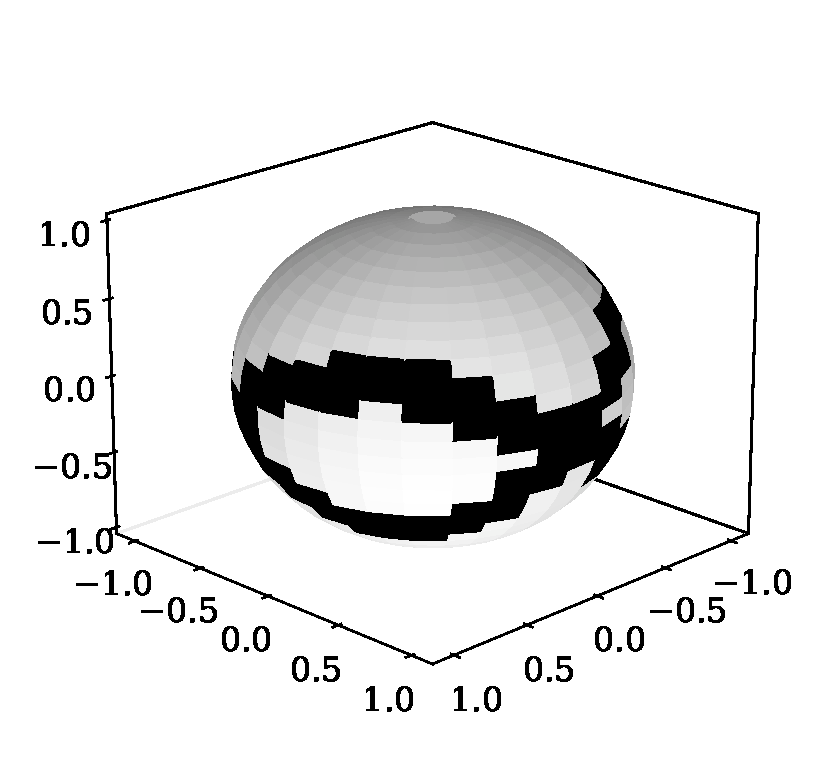
\includegraphics[width=0.35\textwidth]{figs/pi_walk.eps}}\\
\caption{Слева: области на сфере, справа: полученная проекция.}
\label{fg:sp_mesh}
\end{figure}

По полученному разбиению $\mathbb{A}^{p-1}$ на сфере и по точкам фазовой траектории строится функция проекции $\pi(\mathbf{a}), \mathbf{a} \in \mathbb{A}^{p-1}$

\begin{equation}
    \pi(\mathbf{a}) =
    \begin{cases}
	1, & \mbox{если } \mathbf{a} \in \mathbb{A}^{p-1} \cap \mathbf{S}_{z}^{p},\\
    0, & \mbox{если } \mathbf{a} \in \mathbb{A}^{p-1} \setminus \mathbf{S}_{z}^{p}.
    \end{cases}
\label{eq:f_real}
\end{equation}
Пример проекции справа на Рис.~\ref{fg:sp_mesh}.

Составляется система относительно весовых коэффициентов $w_{l_{p-1},...,l_1}$ 

\begin{equation}
\begin{pmatrix} 
	{Y}_{l_{p-1},...,l_1}({\mathbf{a}}_1) & \ldots & {Y}_{0,...,0}({\mathbf{a}}_1)\\
	\vdots& \ddots & \vdots\\
	{Y}_{l_{p-1},...,l_1}({\mathbf{a}}_d) & \ldots & {Y}_{0,...,0}({\mathbf{a}}_d)\\
\end{pmatrix}
\begin{pmatrix} 
	w_{l_{p-1},...,l_1}\\
	\vdots\\
	w_{0,...,0}\\
\end{pmatrix}
=
\begin{pmatrix} 
	\pi(\mathbf{a}_1)\\
	\vdots\\
	\pi(\mathbf{a}_d)\\
\end{pmatrix},
\label{eq:sp_app_matrix}
\end{equation}
\noindentгде $Y_{l_{p-1},...,l_1}({\mathbf{a}}_i)$ --- значение сферической гармоники в точке ${\mathbf{a}}_i$, $d$ --- количество точке в сетке на сфере Рис.~\ref{fg:sp_mesh}.
В более короткой записи:
\begin{equation}
\mathbf{\Pi} = \mathbf{w}_{\text{sp}}^{\mathsf{T}}\mathbf{{Y}}.
\label{eq:sp_app_matrix_short}
\end{equation}

Эта постановка сводит решения к МНК, что ускоряет процедуру расчета весовых коэффициентов.
В силу экспоненциального роста числа сферических гармоник при повышении размерности фазового пространства, вводятся регуляризаторы

\begin{equation}
    \mathbf{\hat{w}}_{\text{sp}} = \text{argmin}_{\mathbf{w}_{\text{sp}}}
    \|\mathbf{{Y}}\mathbf{w}_{\text{sp}} - \mathbf{\Pi}\|^2 + \lambda\|\mathbf{w}_{\text{sp}}\|^2.
\label{eq:arg_l2}
\end{equation}
Решение представимо аналитически:
\begin{equation}
    \mathbf{\hat{w}}_{\text{sp}} = (\lambda \mathbf{I} - \mathbf{{Y}}^{\mathsf{T}}\mathbf{{Y}})^{-1}\mathbf{{Y}}^{\mathsf{T}}\mathbf{\Pi}.
\label{eq:arg_l2_solution}
\end{equation}


%%%%%%%%%%%%%%%%%%%%%%%%%%%%%%%%%%%%%%%%%%%%%%%%%%%%%%%%%%%%%%%%%%%%%%%%%%%%%
\section{Модель классификации весовых коэффициентов}

\begin{figure}[H]
\centering
\captionsetup{justification=centering,margin=2cm}
\subfloat[Классификации с совместной матрицей PCA для всех классов]
{\includegraphics[scale=0.5]{figs/PCA_SVM.pdf}}\\
\subfloat[Классификации с отдельной матрицей PCA для каждого класса]
{\includegraphics[scale=0.5]{figs/TWO_UNIQUE_PCA_SVM.pdf}}\\
\subfloat[Предложенный метод классификации]
{\includegraphics[scale=0.5]{figs/PCA_HARM_SVM.pdf}}\\
\caption{Сравнение различных подходов к классификации фазовой траектории}
\label{fg:alternative_piplines}
\end{figure}

Полученные весовые коэффициенты~(\ref{eq:arg_l2_solution}) для каждого $\mathbf{s} \in \mathbf{S}^{b}$ используются в качестве признакового описания в задаче классификации. Для классификации используется метод опорных векторов с мягким зазором
 
\begin{equation}
    g(\mathbf{w}_{\text{sh}}) = \text{sign}(\mathbf{{w}}_{\text{svm}}^{\mathsf{T}}\,\mathbf{w}_{\text{sh}}).
\label{eq:svm}
\end{equation}

Весовые коэффициенты $\mathbf{{w}_{\text{svm}}}$~(\ref{eq:svm}) оптимизируются

\begin{equation}
\begin{cases}
    \frac{1}{2}\|\mathbf{{w}_{\text{svm}}}\|_2^2 + C\sum_{i=1}^{\hat{m}}\xi_i \xrightarrow{} \min_{{w}_{\text{svm}},\,\xi}\\
    y_i \cdot \mathbf{{w}}_{\text{svm}}^{\mathsf{T}}\mathbf{w}_{\text{sh },i} \geq 1 - \xi_i, \quad i = 1,\dots,b\\
    \xi_i \geq 0, \quad i = 1,\dots,b,\\
\end{cases}
\label{eq:svm_solutin}
\end{equation}
где $C$~---~параметр настройки метода, который позволяет регулировать отношение между максимизацией ширины разделяющей полосы и минимизацией суммарной ошибки, $\xi_i$~---~величина, характеризующая ошибку на объектах ${w}_{\text{svm }i}$. 
\newpage
%%%%%%%%%%%%%%%%%%%%%%%%%%%%%%%%%%%%%%%%%%%%%%%%%%%%%%%%%%%%%%%%%%%%%%%%%%%%%
\section{Модель классификации точек фазовой траектории}

В качества альтернативы используется ближайшая по архитектуре модель описанная в~\cite{Frank_2010}.
В этой работе классифицируются точки фазовой траектории $\mathbf{H}_{x}^{p}$ по стратегии One-Vs-Rest.
Решается задача
\begin{equation}
    g(\mathbf{x}) = \text{sign}(\mathbf{{w}}_{\text{svm}}^{\mathsf{T}}\,\mathbf{x}),
    \quad
    \mathbf{x} \in \mathbf{H}_{x}^{p}.
\label{eq:alternative_svm}
\end{equation}

Сравниваются два варианта классификации.
В первом матрица преобразования метода главных компонент~(\ref{eq:PCA}) строится для объединения всех фазовых траекторий полученных методом задержек и далее классифицируется для каждого класса отдельным методом опорных векторов как показано на Рис.~\ref{fg:alternative_piplines}а.
Во втором варианте матрица преобразования метода главных компонент строится для каждого класса отдельно и далее классифицируется аналогично первому варианту как показано на Рис.~\ref{fg:alternative_piplines}б.

% \begin{figure}[h]
%     \centering
%     \includegraphics[scale=0.5]{./figs/PCA_SVM.pdf}
%     \caption{Схема первой версии метода классификации фазовой траектории}
%     \label{fg:alternative_pipline_v1}
% \end{figure}

% \begin{figure}[h]
%     \centering
%     \includegraphics[scale=0.5]{./figs/TWO_UNIQUE_PCA_SVM.pdf}
%     \caption{Схема второй версии метода классификации фазовой траектории}
%     \label{fg:alternative_pipline_v2}
% \end{figure}
\newpage
%%%%%%%%%%%%%%%%%%%%%%%%%%%%%%%%%%%%%%%%%%%%%%%%%%%%%%%%%%%%%%%%%%%%%%%%%%%%%
\section{Выбор моделей прогнозирования с помощью сферических гармоник}

По временному ряду $\mathbf{s}$ строится траекторная матрица
\begin{equation*}
    \mathbf{H}_{s}^{n} = 
    \begin{bmatrix} 
    	s_{1} & s_{2} & \ldots &s_{n-1} &s_{n}\\
    	s_{2} & s_{3} & \ldots &s_{n} &s_{n+1}\\
    	\vdots& \vdots & \ddots & \vdots & \vdots\\
    	s_{N-n+1} & s_{N-n+2} &\ldots&s_{N-1} &s_{N}\\
    \end{bmatrix} = 
	\begin{bmatrix} 
      	\mathbf{s}_{1}\\
      	\mathbf{s}_{2}\\
      	\vdots\\
      	\mathbf{s}_{m}\\
   \end{bmatrix},
\label{eq:hankel_matri_2}
\end{equation*}
где $m = N-n+1$ --- число строк, $N$~---~длина временного ряда, $n$~---~ширина окна, не меньшая, чем предполагаемый период,  $\mathbf{s}_t=[s_{t},s_{t+1},\ldots,s_{t+n-1}] \in \mathbb{H}_{s} \subseteq \mathbb{R}^{n}$ --- векторы, образующие фазовую траекторию ряда $\mathbf{s}$.

По полученной матрице $\mathbf{H}_{s}^{n}$ строится модель аппроксимации сферическими гармоник, как описано в разделе "Модель фазовой траектории".

Для интерпретации значений модели как вероятности принадлежности вносятся два изменения.
К модели применяется функция сигмоиды $\sigma(x) = \frac{1}{1 + e^{-x}}$:

\[
	f_{\text{sh}}(\mathbf{w}_{\text{sp}},\mathbf{a}) = \sigma\left(
	\sum_{l_{p-1} = 0}^{N_{\text{approx}}}
	\dots
	\sum_{l_1 = -l_2}^{l_2}
	w_{l_{p-1},...,l_1} Y_{l_{p-1},...,l_1}(\mathbf{a})\right),
\]
где $l_{p-1},...,l_1$~---~индексы, определяющие сферические гармоники, $N_{\text{approx}}$~---~максимальное значения старшего индекса, $Y_{l_{p-1},...,l_1}(\mathbf{a})$~---~ сферические гармоники, $w_{l_{p-1},...,l_1}$~---~ весовые коэффициенты.

Оптимизационная задача в обозначениях~(\ref{eq:sp_app_matrix_short}) :
\begin{equation}
    \mathbf{\hat{w}}_{\text{sp}} = \arg \max_{\mathbf{w}_{\text{sp}}}
    \sum_{i = 0}^{d}
    \pi(\mathbf{a}_i)\cdot\text{ln}\big(\sigma(\mathbf{w}_{\text{sp}}^{\mathsf{T}}\mathbf{{Y}}_i)\big) +
    \big(1 - \pi(\mathbf{a}_i)\big)\cdot\text{ln}\big(1 - \sigma(\mathbf{w}_{\text{sp}}^{\mathsf{T}}\mathbf{{Y}}_i)\big)
\label{eq:arg_logreg}
\end{equation}
\noindentгде $\mathbf{{Y}}_i$~---~строка матрицы~(\ref{eq:sp_app_matrix_short}), $d$ --- количество областей разбиения на сфере.

С помощью выбранной модели прогнозирования $g$ получаются $m_s$ последовательных прогнозов будущих значений $\mathbf{\hat{s}} = [\hat{s}_1,...,\hat{s}_{m_s}]$.
По спрогнозированным значениям строится траекторная матрица:
\begin{equation*}
    \mathbf{\hat{H}}_{s}^{n} = 
    \begin{bmatrix} 
    	s_{N-n+1} & s_{N-n+2} &\ldots&s_{N-1} &\hat{s}_{1}\\
    	s_{N-n+2} & s_{N-n+3} &\ldots&\hat{s}_{1} &\hat{s}_{2}\\
    	\vdots& \vdots & \ddots & \vdots & \vdots\\
    	\hat{s}_{m_s-n+1} & \hat{s}_{m_s-n+2} &\ldots&\hat{s}_{m_s-1} &\hat{s}_{m_s}\\
    \end{bmatrix}
\end{equation*}

К полученной матрице $\mathbf{\hat{H}}_{s}^{n}$ применяется матрица преобразований метода главных компонент, полученная ранее при понижении размерности пространства траекторной матрицы на реальных данных, и переход в сферические координаты
\[
\mathbf{\hat{H}}_{x}^{p} = \mathbf{\hat{H}}_{s}^{n} \mathbf{U},\quad \mathbf{S}_{r}^{p} = \phi(\mathbf{H}_{x}^{p}).
\]
Далее для каждой точки фазовой траектории с помощью функции аппроксимации $f_{\text{sh}}$ ставится в соответствие значение
\[
\hat{p} = \hat{p}(\hat{s}|t).
\]
Оно интерпретируется как вероятность принадлежности точки фазовой траектории к области возможных значений по имеющейся предыстории ряда $\mathbf{{s}}$.

Так схема получения оценок вероятности выглядит следующим образом:
\begin{figure}[H]
    \centering
    \captionsetup{justification=centering,margin=2cm}
\[
\xymatrix{
  t \ar[r] &
  \mathbf{s} \ar[r] &
  \mathbf{H}_{s}^{n} \ar[d] \ar[rrr]^{g(\cdot)} &&&
  \mathbf{\hat{s}} \ar[llld]
  \\
  &&
  \mathbf{\hat{H}}_{s}^{n} \ar[r]&
  \mathbf{\hat{S}}_{r}^{p} \ar[rr]^{f_{\text{sp}}(\cdot)}&&
  \mathbf{\hat{p}}
}
\]
\caption{Схема модели предсказания будущих значений временного ряда и оценки их соответствия предыстории.}
\end{figure}

По временному ряду $\mathbf{s}$ строится матрица задержек $\mathbf{H}_{s}^{n}$.
На матрице $\mathbf{H}_{s}^{n}$ настраиваются параметры моделей прогнозирования $g \in G$ и модель аппроксимации $f_{\text{sp}}(\cdot)$.
По прогнозам модели $g$ строится задержек над прогнозами $\mathbf{\hat{H}}_{s}^{n}$.
Такой подход позволяет получить оценку соответствия фазовой траектории  $\mathbf{\hat{p}}=[\hat{p}_1,...,\hat{p}_{m_s}]$ для каждой спрогнозированной точки $\mathbf{\hat{s}}=[\hat{s}_1,...,\hat{s}_{m_s}]$ для каждой модели $g \in G$.
Причем для всех моделей функция аппроксимации $f_{\text{sh}}(\cdot)$ и матрица метода главных компонент $\mathbf{U}$ одни и те же.
\begin{figure}[H]
    \centering
    \captionsetup{justification=centering,margin=2cm}
\[
\begin{pmatrix} 
	\{\mathbf{\hat{s}}_1, \mathbf{\hat{p}}_1\}\\
	\vdots\\
    \{\mathbf{\hat{s}}_{m_{g}}, \mathbf{\hat{p}}_{m_{g}}\}\\
\end{pmatrix}
\xrightarrow{
    \quad
    \text{Decision Rule}
    \quad
}
\mathbf{\hat{s}}_{\text{selected}}
\xrightarrow{}
g_{\text{selected}}
\]
\caption{Схема выбора и/или агрегирования моделей согласно предсказаниями и их оценкам их соответствия предыстории.}
\end{figure}

По полученному множеству $\mathbf{\hat{p}}=[\hat{p}_1,...,\hat{p}_{m_s}]$ для каждой модели считается логарифм правдоподобия.

\begin{equation*}
 L(\hat{s}|t) =  \sum_{i = 1}^{m_s}ln\big(\hat{p}_i(\hat{s}|t)\big)
\end{equation*}

Так для каждой модели $g \in G$  ставится в соответствие логарифм правдоподобия.  
Выбирается та модель, у которой логарифм правдоподобия больше. Для соответствия начальной постановке --- минимальное значение отрицательного логарифма правдоподобия.

\begin{equation*}
g_{\text{selected}} = \arg \min_{g \in G} -L(\hat{s}|t,g,s)
\end{equation*}

Подобное ранжирование интерпретируется как соответствие прогнозов уже имеющейся предыстории.

\newpage
%%%%%%%%%%%%%%%%%%%%%%%%%%%%%%%%%%%%%%%%%%%%%%%%%%%%%%%%%%%%%%%%%%%%%%%%%%%%%
\section{Альтернативные методы выбора моделей прогнозирования}

Для сравнения применяются три вида информационных критериев учитывающих количество параметров моделей и их точность на выборке для обучения.
Обозначения в формулах ниже $RSS$~---~остаточная сумма квадратов, $n$~---~число объектов в выборке, $k$~---~число параметров модели. 

\textbf{Информационный критерий Акаике}~---~это критерий выбора, оценивающий модели с разным числом параметров:
\[
AIC = n\cdot\ln{\frac{RSS}{n-2}} + 2\cdot k
\]

\textbf{Байесовский информационный критерий}, аналогичный AIC, но с более строгим штрафом за количество параметров модели:
\[
BIC = n\cdot\ln{RSS} + k\cdot\ln{n}
\]

\textbf{Mallows’s $C_p$} похожий подход с учетом дисперсии точности среди конечного множества доступных линейных моделей $g \in G$:

\[
C_p = \frac{1}{n}(RSS + 2d\hat{\sigma}^2)
\]
где $d$~---~мощность множества $G$, $\hat{\sigma}^2=\frac{\min_{g \in G}RSS}{n-k-1}$. Считается, что наименьший $RSS$ будет у модели с наибольшим количеством параметров.
\newpage
%%%%%%%%%%%%%%%%%%%%%%%%%%%%%%%%%%%%%%%%%%%%%%%%%%%%%%%%%%%%%%%%%%%%%%%%%%%%%
\section{Эксперимент по классификации сферическими гармониками}

Задан набор данных, измеренный датчиками акселерометра телефона.
Он собирается с частотой дискретизации 50~Гц.
Двадцать четыре участника разного пола, возраста, веса и роста выполнили три типа повторяемых физических активностей: движение по лестнице, ходьба, бег.
Более подробное описание набора данных в~\cite{Malekzadeh_2018}.

Участники имеют разные типы походки и, как следствие, разные фазовые траектории.
Поэтому были отобраны три человека со схожими показателями роста и веса.

Алгоритм классификации схож с вариантом на Рис.~\ref{fg:alternative_piplines}б. Основное отличие в аппроксимация фазовой траектории линейной комбинацией сферических гармоник как показано на Рис.~\ref{fg:alternative_piplines}в.

Размер предыстории выбирается равным $n = 150$, что советует трем секундам.
Период движений в данных не превосходит двух с половиной секунд.

Значение старшего индекса, используемого для построения модели сферических~(\ref{eq:f_sh}) гармоник, выбирается равным $N_{\text{approx}} = 10$ для размерности фазового пространства $\mathbf{H}_{x}^{p}$ равного трем, $N_{\text{approx}} = 6$ для размерности четыре и $N_{\text{approx}} = 3$ для размерности пять.
Для пространств большей размерности эксперимент не проводился из-за малого объема данных и  вычислительной неэффективности подсчета сферических гармоник для размерности пространства равной шести и более.

\begin{table}[H]
% \centering
% \captionsetup{margin=1cm}
    \caption{F-score классификации на трех пользователях с одинаковым типом фазовой траектории}
    \label{tbl:accuracy_table_all}
    \centering\medskip\tabcolsep=6pt\small
    \begin{tabular}{|l||ccc|ccc|ccc|}
    \hline
        Метод
            & \multicolumn{3}{c|}{Ходьба}
            & \multicolumn{3}{c|}{Бег}
            & \multicolumn{3}{c|}{Лестница}\\
    \hline\hline
        Размерность $p$
            & 3 & 4 & 5
            & 3 & 4 & 5
            & 3 & 4 & 5\\
    \hline
        {Пользователь 1}
            & $0.98$ & $0.99$ & $0.95$ % Ходьба
            & $0.97$ & $0.99$ & $0.8$ % бег
            & $0.86$ & $0.84$ & $0.92$ \\% Лестница
    \hline
        {Пользователь 2}
            & $0.99$ & $0.97$ & $0.57$ % Ходьба
            & $0.98$ & $0.98$ & $0.91$ % бег
            & $0.95$ & $0.68$ & $0.86$ \\% Лестница
    \hline
        {Пользователь 3}
            & $0.96$ & $0.93$ & $0.58$ % Ходьба
            & $0.89$ & $0.64$ & $0.82$ % бег
            & $0.85$ & $0.65$ & $0.86$ \\% Лестница
    \hline
    \end{tabular}
\end{table}

\begin{figure}[H]
    \centering
    \captionsetup{justification=centering,margin=2cm}
    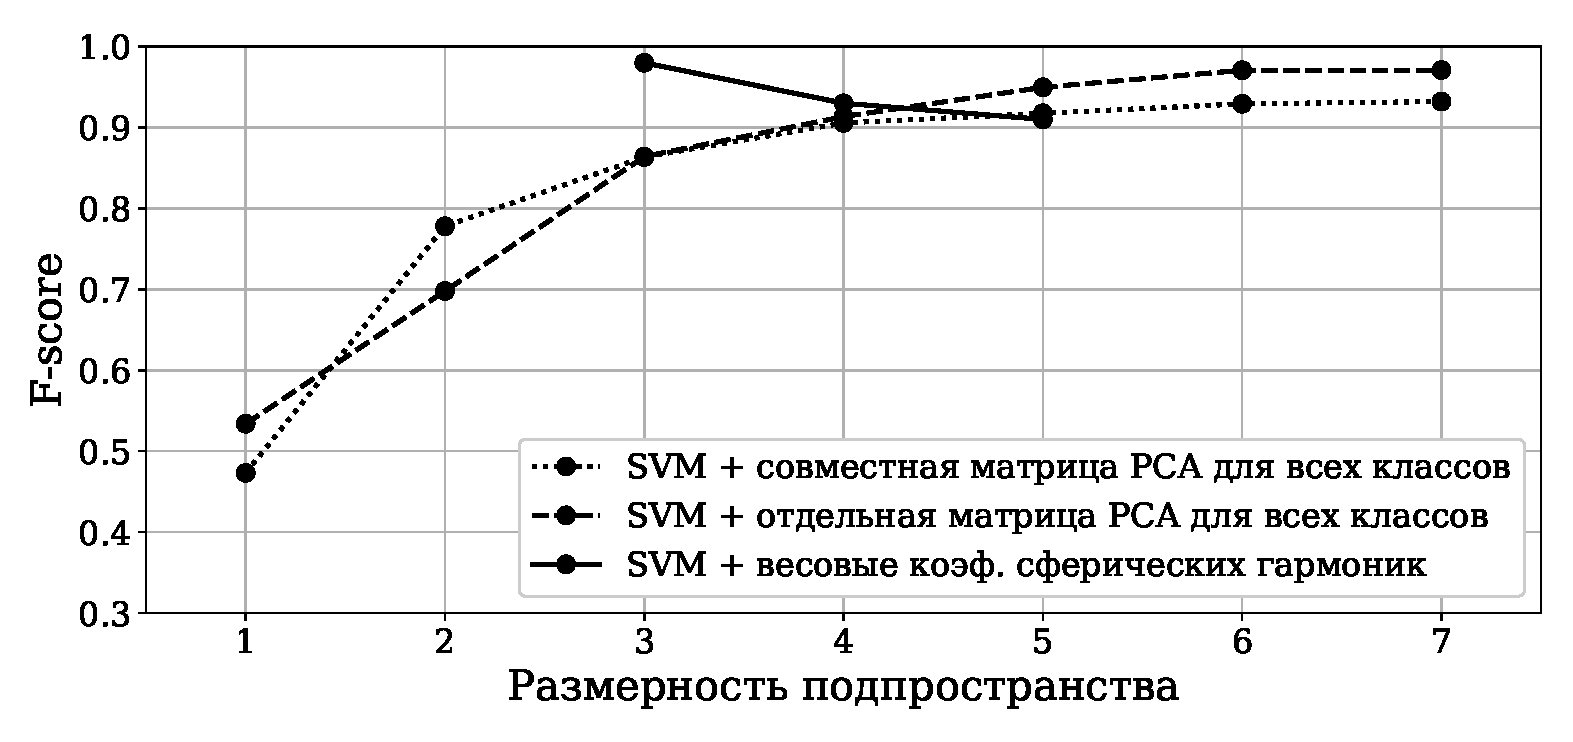
\includegraphics[scale=0.55]{./figs/result_first.eps}
    \caption{F-score на ходьбе, беге, спуску и подъему по лестнице для одного пользователя}
    \label{fg:clf_result_one}
\end{figure}

На Рис.~\ref{fg:clf_result_one} показано качество классификации F-score движении одного человека.
Видно, что для эффективной классификации достаточно трехмерных сферических гармоник.

При применении методов, обученных  на данных первого пользователя, для классификации временных рядов записанных с второго и третьего пользователей качество падает в зависимости от типа движения.
Так бег и ходьба классифицируются лучше, чем движение по лестнице.
В таблице~\ref{tbl:accuracy_table_all} представлена качество классификации для нескольких пользователей.
При этом из-за увеличения размерности пространства падает общее качество классификации.
Средние значения представлены на Рис.~\ref{fg:clf_result_many} и в таблице~\ref{tbl:accuracy_table_mean}.

\begin{table}[H]
    % \centering
    % \captionsetup{margin=2cm}
    \caption{Среднее качество классификации на трех пользователях с одинаковым типом фазовой траектории}
    \label{tbl:accuracy_table_mean}
    \centering\medskip\tabcolsep=12pt\small
    \begin{tabular}{|l||ccc|}
        \hline
        Метод & \multicolumn{3}{c|}{F-score}\\
        \hline\hline
        Размерность $p$ & 3 & 4 & 5\\
        \hline
        {SVM + весовые коэф. сферических гармоник}     & $0.90$ & $0.82$ & $0.81$ \\
        \hline
        {SVM + совместная матрица PCA для всех классов} & $0.79$ & $0.80$ & $0.89$ \\
        \hline
        {SVM + отдельная матрица PCA для каждого класса} & $0.78$ & $0.81$ & $0.81$ \\
        \hline
    \end{tabular}
\end{table}

\begin{figure}[H]
    \centering
    \captionsetup{justification=centering,margin=2cm}
    \includegraphics[scale=0.55]{./figs/result_mean.eps}
    \caption{Средний и СКО F-score на ходьбе, беге, спуску и подъему по лестнице}
    \label{fg:clf_result_many}
\end{figure}

\begin{table}[H]
\centering
\caption{Таблица сравнений разных классов движений}
\begin{tabular}{p{1.1cm}p{3.3cm}p{4.6cm}p{4cm}}
    & Временной ряд
    & Фазовая траектория
    & Модель
    \\
    \hline
    \rotatebox{90}{ \text{Ходьба} }
    & 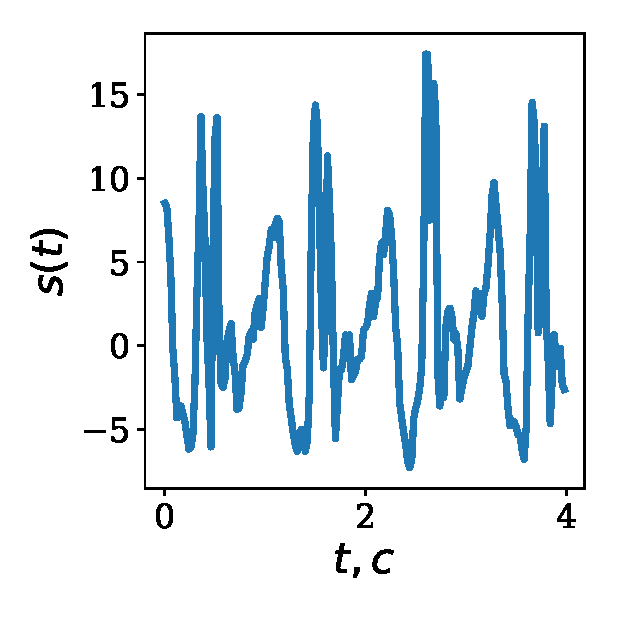
\includegraphics[scale=0.31]{figs/time_series_wlk_8.eps}
    & 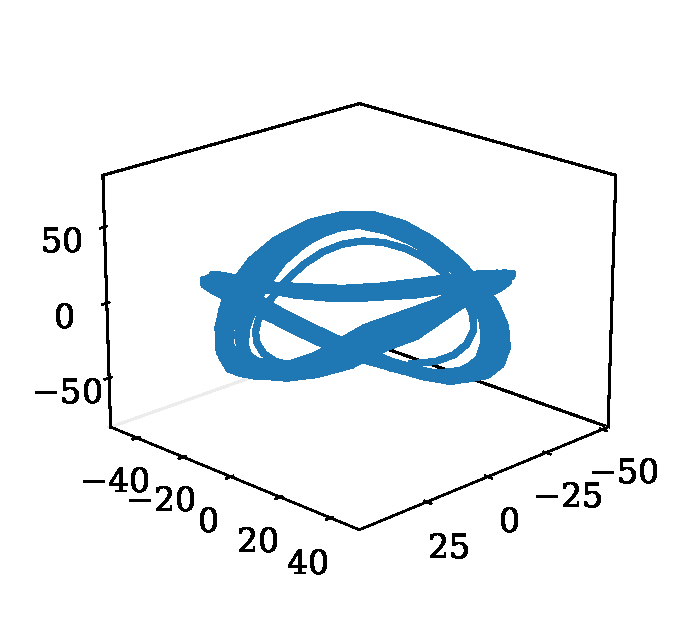
\includegraphics[scale=0.36]{figs/phase_traj_wlk_8.eps}
    & \includegraphics[scale=0.36]{figs/spharm_wlk_8.eps}
    \\ 
    \hline
    \rotatebox{90}{ \text{Бег} }
    & 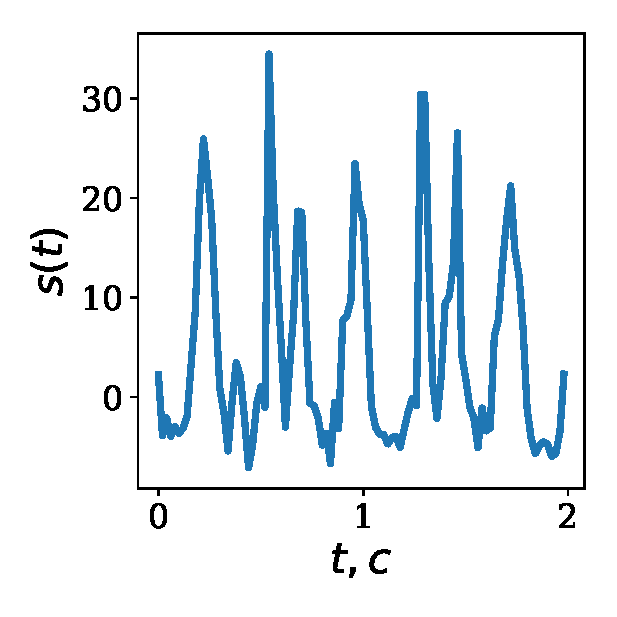
\includegraphics[scale=0.31]{figs/time_series_jog_9.eps}
    & 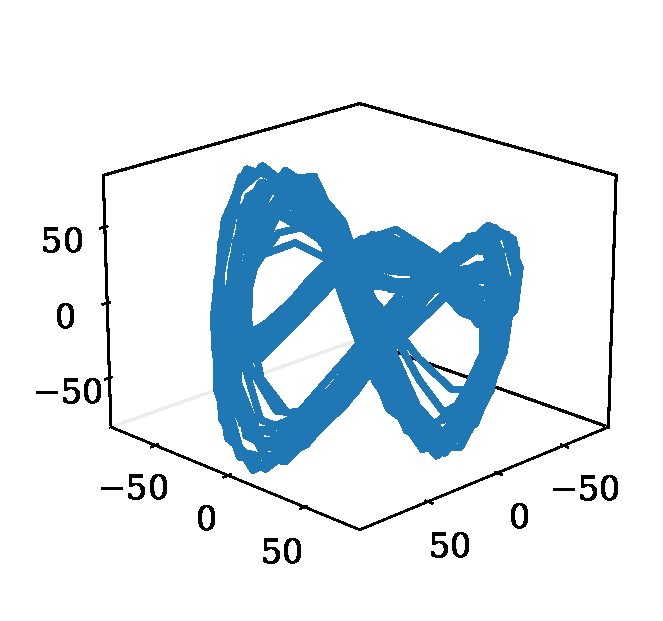
\includegraphics[scale=0.36]{figs/phase_traj_jog_9.eps}
    & \includegraphics[scale=0.36]{figs/spharm_jog_9.eps}
    \\ 
    \hline
    \rotatebox{90}{ \text{Лестница} }
    & 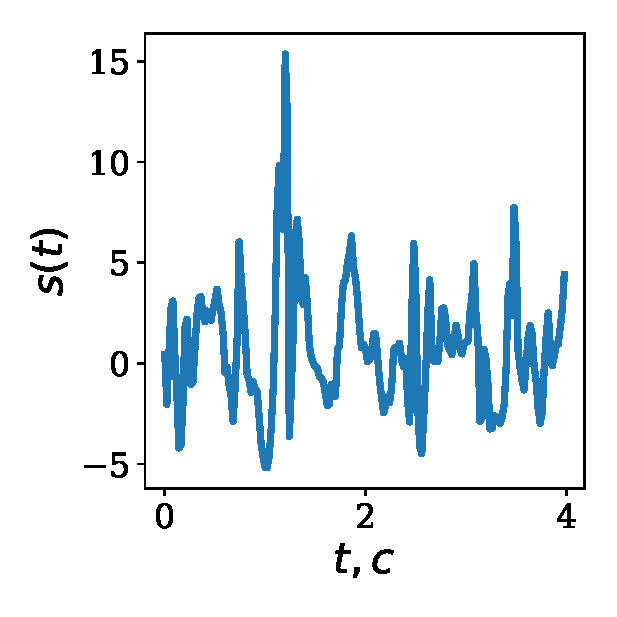
\includegraphics[scale=0.31]{./figs/time_series_ups_4.eps}
    & 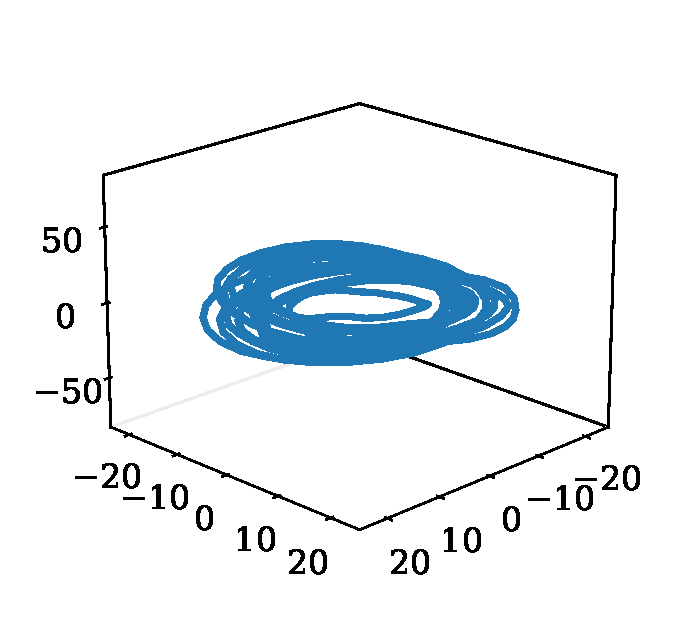
\includegraphics[scale=0.36]{./figs/phase_traj_ups_4.eps}
    & \includegraphics[scale=0.36]{./figs/spharm_ups_4.eps}
    \\ 
    \hline
\end{tabular}
\label{tbl:table_of_figures}
\end{table}

В таблице~\ref{tbl:table_of_figures} показаны результаты работы алгоритма.
Слева фрагмент временного ряда записанного с акселерометра.
По центру полученные фазовые траектории в трехмерном пространстве.
Справа модели сферических гармоник.
Видно, что разные классы временных рядов имеют разные траектории и разные модели аппроксимации.
%%%%%%%%%%%%%%%%%%%%%%%%%%%%%%%%%%%%%%%%%%%%%%%%%%%%%%
%%%%%%%%%%%%%%%%%%%%%%%%%%%%%%%%%%%%%%%%%%%%%%%%%%%%%%
\section{Эксперимент по выбору модели прогнозирования}
\textbf{Данные акселерометра велопрогулки.}
Сигнал был записан с датчика акселерометра во время поездки на велосипеде.
Частота дискретизации ~50Гц.
Для оценки модели применялись оценка RMSE на отложенной выборке, информационные критерии BIC, AIC, Mallow's $\text{C}_p$.  
Врмененной ряд был разделен: 50\%~---~для обучения, 25\%~---~для RMSE методом HoldOut, 25\%~---~для оценки методов выбора модели .
 
\renewcommand{\arraystretch}{1.25}
 
\begin{table}[H]
\caption{Качества ранжирования моделей на профилю велопрогулки}
\centering\medskip\tabcolsep=4pt

\label{tbl:rang_table_bike}
\begin{tabular}{l|ccccccc}
\hline
G &  MSE тест &  MSE отложенная & $\mathbf{\hat{\bar{p}}}$ & $\text{C}_p$ & AIC & BIC \\
\hline
$g_0$ &  9.724991 &  12.343679 &  0.7439 & \textbf{21.188266} & \textbf{1.132565} & \textbf{1.664724} \\
$g_1$ &  9.736825 &  11.796950 &  0.7312 & 21.262064 & 1.136510 & 1.721885 \\
$g_2$ &  9.523704 &  11.495201 &  0.7595 & 21.570077 & 1.152974 & 1.791565 \\
$g_3$ &  \textbf{9.195918} &  \textbf{11.147608} &  \textbf{0.8426} & 21.834579 & 1.167112 & 1.858919 \\
$g_4$ &  \textbf{9.159391} &  \textbf{11.180613} &  \textbf{0.8492} & 22.493779 & 1.202348 & 1.947371 \\
$g_5$ & 11.213219 &  12.465094 &  0.7808 & 24.320765 & 1.300005 & 2.098244 \\
$g_6$ & 10.610619 &  12.381153 &  0.7958 & 24.836478 & 1.327571 & 2.179026 \\
$g_7$ & 11.351968 &  12.014565 &  0.8183 & 25.050591 & 1.339016 & 2.243687 \\
$g_8$ & 12.638967 &  11.746108 &  0.7952 & 25.379346 & 1.356588 & 2.314475 \\
$g_9$ & 13.561436 &  12.335483 &  0.8161 & 24.528546 & 1.311111 & 2.322214 \\
\hline
\end{tabular}
\end{table}

Как видно из таблицы~\ref{tbl:rang_table_bike} предложенный методу лучше ранжирует модели и выделяет более точную модель в будущем.
Близким по точности методом является оценка качества на отложенной выборке.
Информационные критерии показали.

\begin{figure}[H]
    \centering
    \captionsetup{justification=centering,margin=2cm}
    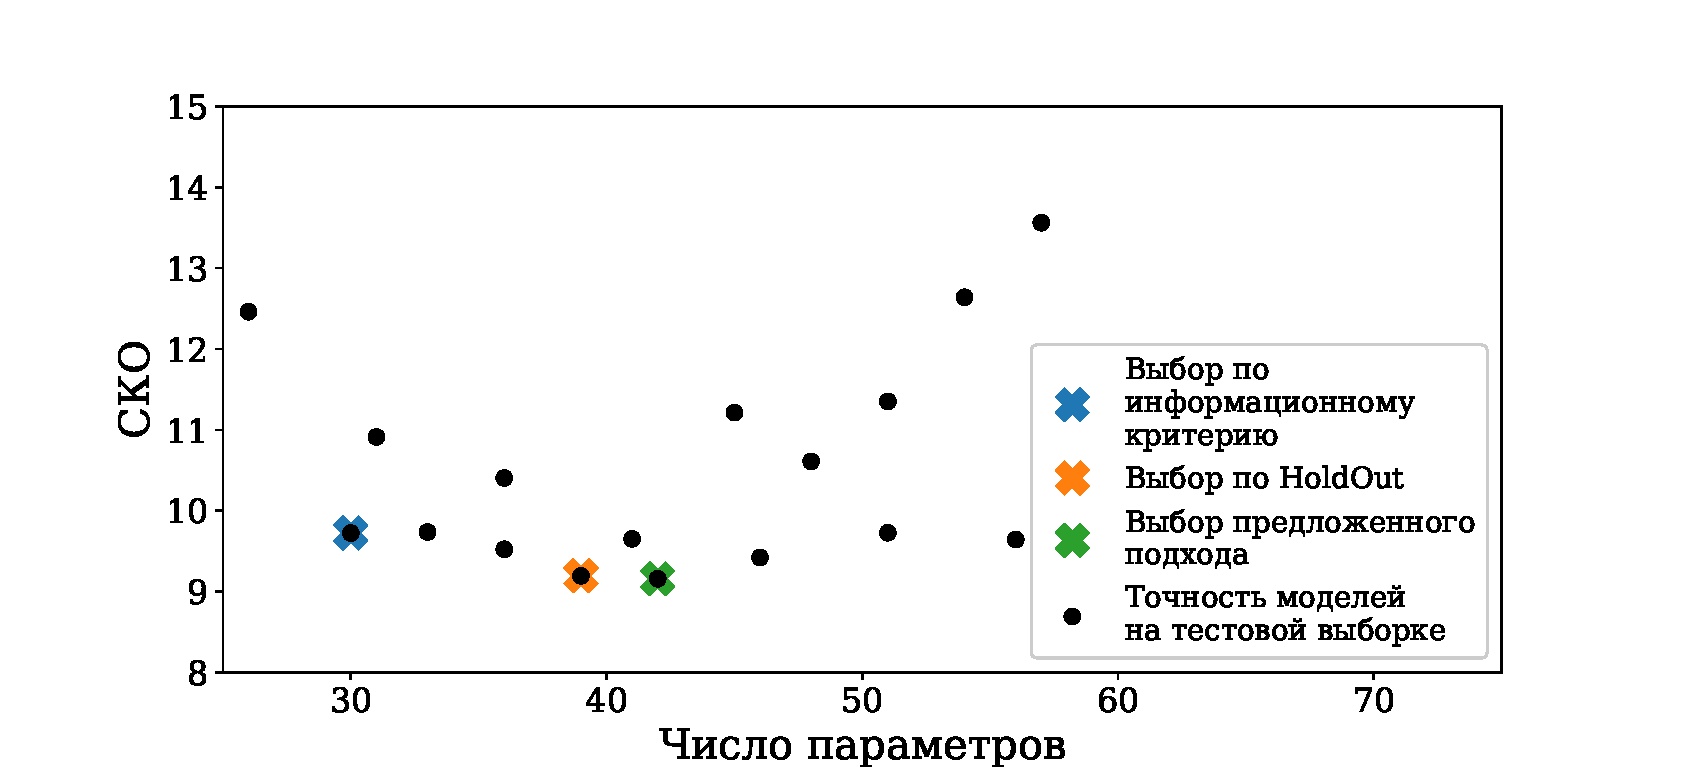
\includegraphics[scale=0.6]{figs/pareto_fig.eps}
    \caption{СКО моделей на тестовой выборке}
    \label{fg:select_pareto}
\end{figure}

На  из Рис.~\ref{fg:select_pareto} видно, что предложенный метод и информационные критерии выбирают оптимальный по Парето модели.
Предложенный метод выбирает более точные модели.
Информационные критерии выбирает более простые модели.

\begin{figure}[h]
    \centering
    \captionsetup{justification=centering,margin=1cm}
    {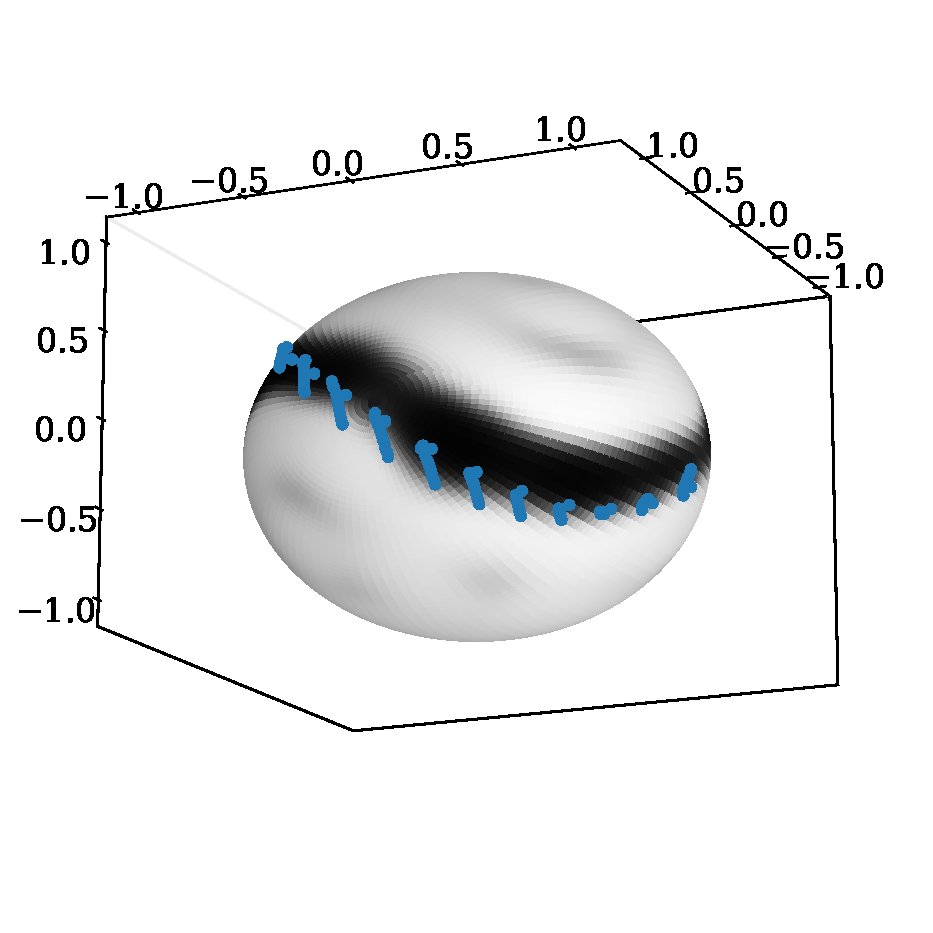
\includegraphics[width=0.45\textwidth]{figs/IC_model.eps}}
    {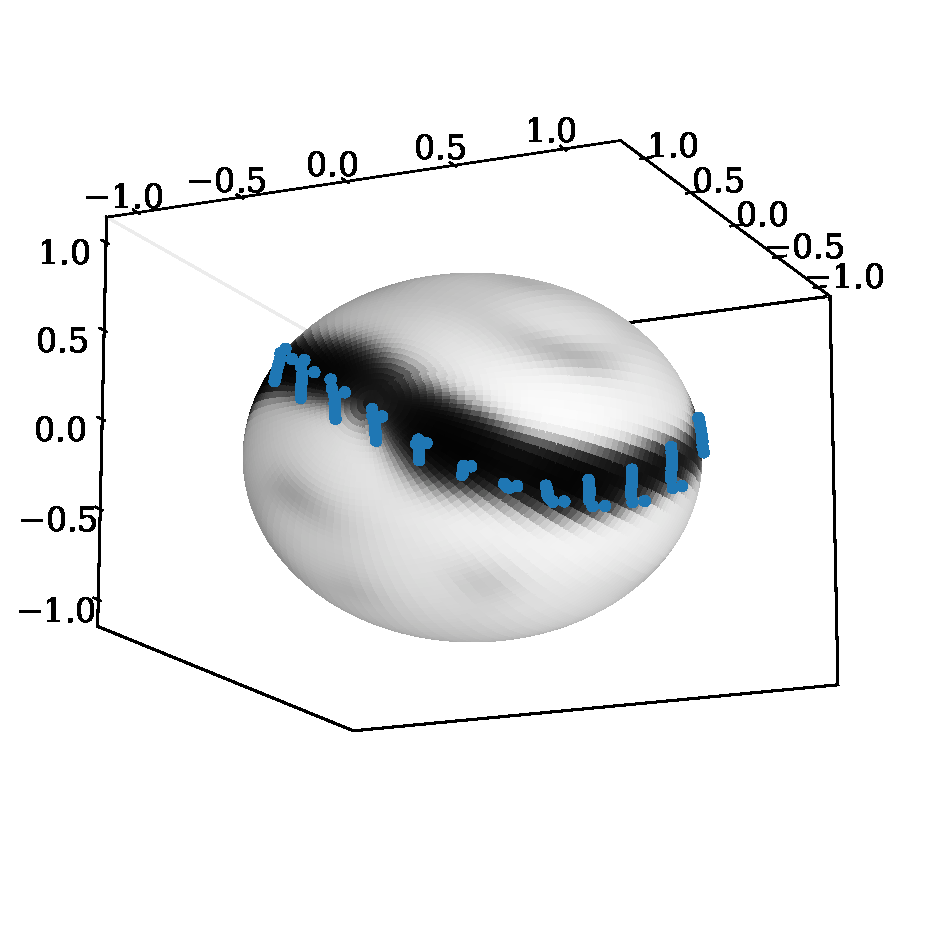
\includegraphics[width=0.45\textwidth]{figs/P_model.eps}}\\
    \caption{Слева: выбранная модель по информационным критериям, справа: выбранная модель по предложенному методу и HoldOut.}
\label{fg:P_IC_model}
\end{figure}

Как видно из Рис.~\ref{fg:P_IC_model} выбранные модели согласно информационным критериям имеют менее вероятную фазовую траекторию.
Предложенный метод выбирает более вероятную фазовую траекторию так, чтобы больше точке лежало в области дисперсии.
% \textbf{Данные потребления энергии.}

\textbf{Датасет физической активности.}
Эксперимент проведен на данных из~\cite{Malekzadeh_2018}.
Данные --- это показатели акселерометра с мобильных устройств десяти пользователей по профилю ходьбы и бега на двух разных маршрутах .
Для корректной оценки ошибки среднеквадратичная ошибка MSE была заменена на коэффициент детерминации R$^2$.
Так амплитуда временного ряда не влияет на сравнительный анализ сравнительный анализ.
Для каждого временного ряда считается $\Delta \text{R}^2 = \text{R}^2_{\text{лучшая}} - \text{R}^2_{\text{выбранная}}$.
$\text{R}^2_{\text{лучшая}}$ --- лучшее значение прогнозов на тестовой выборке.
$\text{R}^2_{\text{выбранная}}$ --- значение прогнозов выбранной модели на тестовой выборке.
Для каждого метода выбора модели считается Средний и СКО $\Delta \text{R}^2$.

\begin{table}[H]
\caption{Качества ранжирования на данных физической активности}
\centering\medskip\tabcolsep=6pt
\label{tbl:rang_table}
\begin{tabular}{l|ccccc}
\hline
 &  HoldOut&  $\mathbf{\hat{\bar{p}}}$&  AIC &  BIC & Mallow's $\text{C}_p$\\
\hline 
Точность выбора            &   0.31 &  0.34 & 0.26 & 0.22 & 0.26 \\
Средний $\Delta \text{R}^2$&   0.11 &  0.09 & 0.11 & 0.10 & 0.11 \\
СКО $\Delta \text{R}^2$    &   0.19 &  0.15 & 0.17 & 0.16 & 0.17 \\
\hline
\end{tabular}
\end{table}

Как видно из таблицы~\ref{tbl:rang_table} предложенный метод в среднем лучше выбирает модели.
Чем больше точность и чем меньше средний $\Delta \text{R}^2$ тем лучше.
Предложенный метод в среднем лучше выбирает модели.
Это происходит в силу хорошей настройки модели аппроксимации.
На временных рядах с базовыми настройками гиперпараметров модели аппроксимации фазовой траектории качество выбора модели хуже, чем у метода HoldOut и информационных критериев.
Это связано с наличием в временных рядах разладки.
Так изменится характера движения, то изменится вид фазовой траекории.
Метод является чувствительным  к изменению с быстрой ходьбы на прогулочную.

\newpage
%%%%%%%%%%%%%%%%%%%%%%%%%%%%%%%%%%%%%%%%%%%%%%%%%%%%%%
%%%%%%%%%%%%%%%%%%%%%%%%%%%%%%%%%%%%%%%%%%%%%%%%%%%%%%
\section*{Заключение}
\addcontentsline{toc}{section}{Заключение}
Был предложен метод построения фазового пространства.
В сферических координатах была построена модель аппроксимации, как линейная комбинация сферических гармоник.
Модель аппроксимации сохраняет геометрическую структуру фазовой траектории временного ряда и интерпретируется как вероятность принадлежности точки фазовой траектории к предыстории.

Вычислительные эксперименты показали, что параметры данной модели имеют лучшую разделяющую способность при меньшей размерности подпространства, чем ближайший метод.
При меньшем количестве настраиваемый параметров качество лучше.
Предложенный метод выбора модели прогнозирования показал лучшее качество ранжирования в сравнении с оценкой на отложенной выборке и информационными критериями BIC, AIC, Mallow's $\text{C}_p$.

Однако для большей эффективности метод требует сложной настройки и больший размер обучающей выборки, чем альтернативные методы.
При невозможности настроить гиперпараметры модели качество хуже.
Предложенный метод оказывается излишне чувствительным к изменению характера походки. 
Так у разных пользователей могут быть разные типы фазовых траекторий для одного типа движения.
Подобные особенности будут рассмотрены в будущих работах.
\newpage
%%%%%%%%%%%%%%%%%%%%%%%%%%%%%%%%%%%%%%%%%%%%%%%%%%%%%%
%%%%%%%%%%%%%%%%%%%%%%%%%%%%%%%%%%%%%%%%%%%%%%%%%%%%%%
\addcontentsline{toc}{section}{Список литературы}
\addtocontents{toc}{\protect\setcounter{tocdepth}{-1}}
% \nocite{*}
\bibliographystyle{plain}
\bibliography{biblio.bib}

\end{document}